\documentclass[a4paper,11pt]{article}
\input{/home/tof/Documents/Cozy/latex-include/preambule_doc.tex}
\input{/home/tof/Documents/Cozy/latex-include/preambule_commun.tex}
\newcommand{\showprof}{show them}  % comment this line if you don't want to see todo environment
\setlength{\fboxrule}{0.8pt}
\fancyhead[L]{\fbox{\Large{\textbf{Routage 04}}}}
\fancyhead[C]{\textbf{Open Shortest Path First}}
\newdate{madate}{10}{09}{2020}
%\fancyhead[R]{\displaydate{madate}} %\today
%\fancyhead[R]{Seconde - SNT}
%\fancyhead[R]{Première - NSI}
\fancyhead[R]{Terminale - NSI}
\fancyfoot[L]{\vspace{1mm}Christophe Viroulaud}
\AtEndDocument{\label{lastpage}}
\fancyfoot[C]{\textbf{Page \thepage/\pageref{lastpage}}}
\fancyfoot[R]{\includegraphics[width=2cm,align=t]{/home/tof/Documents/Cozy/latex-include/cc.png}}
\usepackage{tikz}

\begin{document}
\section{Problématique}
Le protocole RIP souffre de plusieurs limitations :
\begin{itemize}
    \item Il est limité à quinze sauts.
    \item La route la plus courte en nombre de routeurs traversés n'est pas forcément la plus rapide si on prend les débits en compte.
\end{itemize}
\begin{center}
    \framebox{Quelle solution mettre en place pour surmonter ces limitations?}
\end{center}
\section{Bande passante}
\begin{aretenir}[]
La \emph{bande passante} est la quantité d'information qui peut être transmise par unité de temps. Elle se mesure en \emph{bits par seconde (bit/s)}.
\end{aretenir}
Pour obtenir la meilleure route possible, le nombre de routeurs traversés ne sera plus le critère de sélection. On définira maintenant le \emph{coût d'une liaison} pour relier deux routeurs.
\begin{aretenir}[]
Le coût d'une liaison est calculé par la relation :
$$\dfrac{10^8}{\mbox{bande passante}}$$
Dans le cas d'une connexion asymétrique on utilise le débit descendant.
\end{aretenir}
La valeur $10^8$ a été choisie pour donner un coût de 1 à une liaison FastEthernet de 100Mbit/s.
\begin{activite}
Calculer les coûts des connexions suivantes :
\begin{itemize}
    \item satellite 50Mbit/s,
    \item câble Éthernet 10Mbit/s,
    \item modem 62500bit/s,
    \item fibre optique 1Gbit/s,
    \item ADSL 13Mbit/s (descendant), 1Mbit/s (montant).
\end{itemize}
\end{activite}
\section{Open Shortest Path First}
Le protocole OSPF a été développé dans les années 90 pour pallier les difficultés du protocole RIP. La métrique utilisée dépend de la bande passante des connexions. On parle de \textbf{routage à état de lien}.
\subsection{Organisation en zones}
Le protocole OSPF peut être utilisé pour de grands réseaux. Pour diminuer la charge de calcul des routeurs, le réseau est découpé en zones.
\begin{aretenir}[]
    Chaque zone a un numéro unique. La zone 0, obligatoire pour le protocole OSPF, est appelée \textbf{Backbone} est la zone centrale à laquelle toutes les autres zones sont connectées à l'aide d’un routeur particulier appelé \textbf{ABR (Area Border Router)}.
\end{aretenir}
\begin{center}
    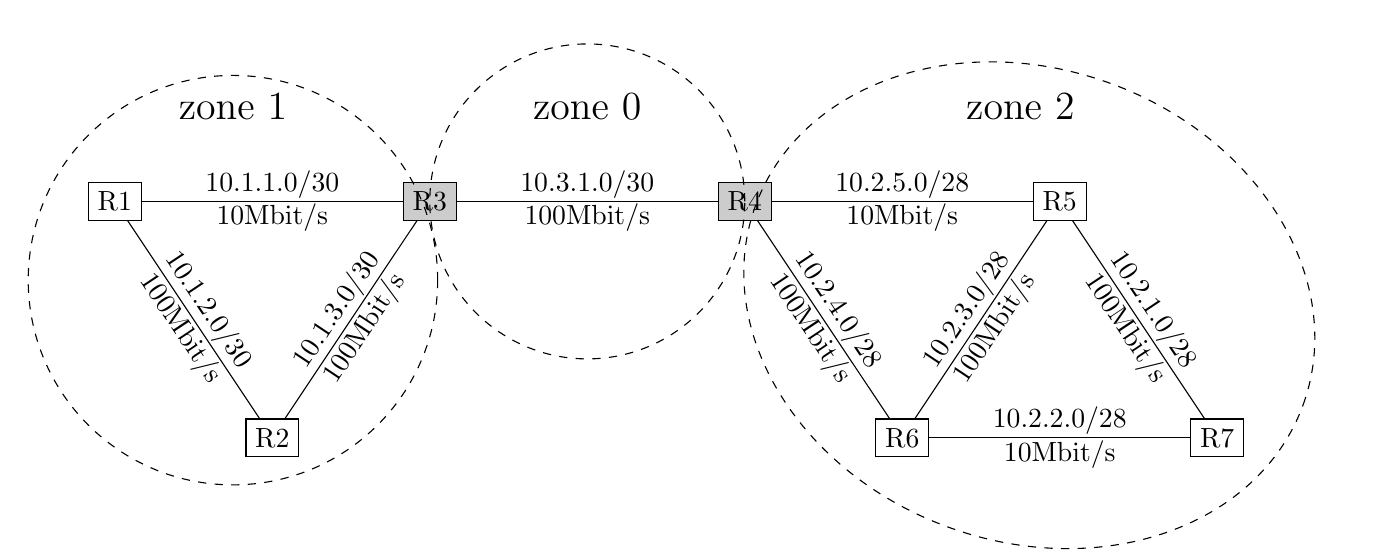
\begin{tikzpicture}
        \node[draw] (R1) at (-6,3) {R1};
        \node[draw] (R2) at (-4,0) {R2};
        \node[draw, fill=gray!40] (R3) at (-2,3) {R3};
        \node[draw, fill=gray!40] (R4) at (2,3) {R4};
        \node[draw] (R5) at (6,3) {R5};
        \node[draw] (R6) at (4,0) {R6};
        \node[draw] (R7) at (8,0) {R7};
        \node (Z1) at (-4.5,4.2) {\Large{zone 1}};
        \node (Z0) at (0,4.2) {\Large{zone 0}};
        \node (Z2) at (5.5,4.2) {\Large{zone 2}};
        
        \draw (R1) -- (R3) node[midway,text width=1.8cm, text centered]{10.1.1.0/30 10Mbit/s};
        \draw (R1) -- (R2) node[sloped, midway,text width=1.8cm, text centered]{10.1.2.0/30 100Mbit/s};
        \draw (R3) -- (R2) node[sloped, midway,text width=1.8cm, text centered]{10.1.3.0/30 100Mbit/s};
        \draw (R3) -- (R4) node[midway,text width=1.8cm, text centered]{10.3.1.0/30 100Mbit/s};
        \draw (R4) -- (R5) node[midway,text width=1.8cm, text centered]{10.2.5.0/28 10Mbit/s};
        \draw (R4) -- (R6) node[sloped, midway,text width=1.8cm, text centered]{10.2.4.0/28 100Mbit/s};
        \draw (R5) -- (R6) node[sloped, midway,text width=1.8cm, text centered]{10.2.3.0/28 100Mbit/s};
        \draw (R7) -- (R6) node[midway,text width=1.8cm, text centered]{10.2.2.0/28 10Mbit/s};
        \draw (R5) -- (R7) node[sloped, midway,text width=1.8cm, text centered]{10.2.1.0/28 100Mbit/s};

        \draw[dashed] (0,3) circle (2) ;
        \draw[dashed] (-4.5,2) circle (2.6) ;
        \draw[dashed,rotate=-20] (4.7,3.5) ellipse (3.7 and 3) ;
    \end{tikzpicture}
    \captionof{figure}{Découpage en zones}
    \label{zone}
\end{center}
\subsection{Découverte du réseau}
\subsubsection{Identificateur}
Chaque routeur choisit un \emph{identifiant unique}. Une stratégie courante est de prendre la plus grande adresse IP parmi celles de ses sous-réseaux.
\begin{activite}
Déterminer un identificateur possible pour chacun des routeurs.
\end{activite}
\begin{aretenir}[Remarque]
Des identificateurs peuvent apparaître en double. Des mécanismes permettent d'identifier et corriger ces erreurs.
\end{aretenir}
\begin{center}
    \framebox{Afin de simplifier les écritures nous conserveront les notations R1\dots 7 pour repérer les routeurs.}
\end{center}
\subsubsection{Message HELLO}
Chaque routeur envoie ensuite des paquets de type \emph{HELLO} à travers toutes ses interfaces. À réception de la réponse il établit une relation de voisinage.
\begin{center}
    \begin{tabular}{|*{4}{c|}}
        \hline
        Lien & Sous-réseau & Coût & Zone \\
        \hline
        R1 - R2 & 10.1.2.0/30 & 1 & 1 \\
        \hline
        R1 - R3 & 10.1.1.0/30 & 10 & 1 \\
        \hline
    \end{tabular}
    \captionof{table}{Relation de voisinage pour R1}
\end{center}
\begin{activite}
Établir le tableau des relations de voisinage pour R5.
\end{activite}
\begin{aretenir}[Remarque]
C'est également lors de cette étape que les routeurs \emph{ABR} annoncent leur rôle aux autres.
\end{aretenir}
\subsubsection{Message LSA}
Les routeurs s'échangent ensuite des paquets \textbf{LSA (Link State Advertisement)} qui contiennent les informations dont ils disposent sur la topologie du réseau. Ces échanges sont \emph{limités à la zone à laquelle appartient le routeur}. Plusieurs échanges de messages LSA sont nécessaires pour synchroniser les connaissances de tous les routeurs.
\begin{center}
    \begin{tabular}{|*{4}{c|}}
        \hline
        Lien & Sous-réseau & Coût & Zone \\
        \hline
        R1 - R2 & 10.1.2.0/30 & 1 & 1 \\
        \hline
        R1 - R3 & 10.1.1.0/30 & 10 & 1 \\
        \hline
        R2 - R3 & 10.1.3.0/30 & 1 & 1 \\
        \hline
    \end{tabular}
    \captionof{table}{Topologie pour R1}
\end{center}
\begin{activite}
Établir la vision de la topologie du réseau pour R5.
\end{activite}
\subsection{Calculs des meilleurs routes}
Connaissant la topologie de sa zone, chaque routeur exécute un algorithme de calcul du plus court chemin vers chaque routeur.
\begin{aretenir}[]
\textbf{L'algorithme de Dijkstra} -établi en 1959- permet de trouver le plus court chemin entre deux sommets d'un graphe pondéré.
\end{aretenir}
\begin{center}
    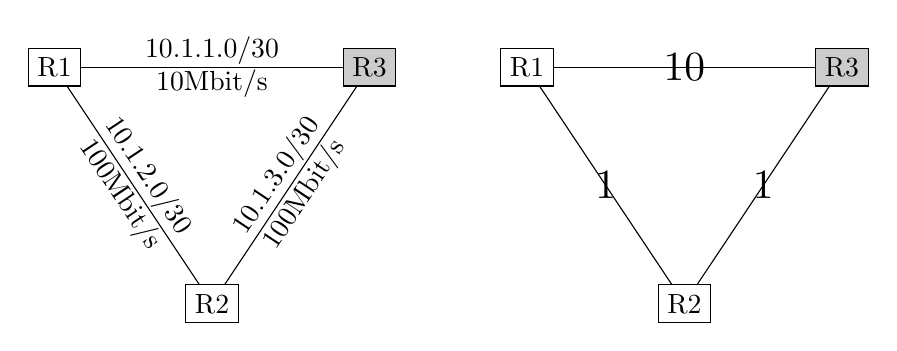
\begin{tikzpicture}
        \node[draw] (R1) at (-6,3) {R1};
        \node[draw] (R2) at (-4,0) {R2};
        \node[draw, fill=gray!40] (R3) at (-2,3) {R3};
        
        \draw (R1) -- (R3) node[midway, scale=1.5]{10};
        \draw (R1) -- (R2) node[midway, scale=1.5]{1};
        \draw (R3) -- (R2) node[midway, scale=1.5]{1};


        \node[draw] (R1b) at (-12,3) {R1};
        \node[draw] (R2b) at (-10,0) {R2};
        \node[draw, fill=gray!40] (R3b) at (-8,3) {R3};
        \draw (R1b) -- (R3b) node[midway,text width=1.8cm, text centered]{10.1.1.0/30 10Mbit/s};
        \draw (R1b) -- (R2b) node[sloped, midway,text width=1.8cm, text centered]{10.1.2.0/30 100Mbit/s};
        \draw (R3b) -- (R2b) node[sloped, midway,text width=1.8cm, text centered]{10.1.3.0/30 100Mbit/s};
    \end{tikzpicture}
    \captionof{figure}{Graphe pondéré de la zone 1}
    \label{zone1}
\end{center}
Le routeur R1 calcule le chemin le plus court pour atteindre chaque réseau de la zone 1.
\begin{center}
    \begin{tabular}{|*{4}{c|}}
        \hline
        Destination & Passerelle & Interface & Coût \\
        \hline
        10.1.2.0/30 &  & 10.1.2.1 & 1 \\
        \hline
        10.1.3.0/30 & 10.1.2.2 (R2) & 10.1.2.1 & 2 \\
        \hline
        10.1.1.0/30 &  & 10.1.1.1 & 10 \\
        \hline
    \end{tabular}
    \captionof{table}{Table de routage de R1}
\end{center}
\begin{aretenir}[Remarque]
Les adresses 10.1.2.1 et 10.1.2.2 correspondent aux interfaces (de respectivement R1 et R2) sur le réseau 10.1.2.0/30.\\
L'adresse 10.1.1.1 correspond à l'interface de R1 sur le réseau 10.1.1.0/30.
\end{aretenir}
Le routeur \emph{de bordure} R3 communique les plus courts chemins (passant par lui) vers la zone 2. Le routeur R1 complète alors sa table de routage.
\begin{center}
    \begin{tabular}{|*{4}{c|}}
        \hline
        Destination & Passerelle & Interface & Coût \\
        \hline
        10.1.2.0/30 &  & 10.1.2.1 & 1 \\
        \hline
        10.1.3.0/30 & 10.1.2.2 (R2) & 10.1.2.1 & 2 \\
        \hline
        10.1.1.0/30 &  & 10.1.1.1 & 10 \\
        \hline
        10.3.1.0/30 & 10.1.2.2 (R2) & 10.1.2.1 & 3 \\
        \hline
        10.2.5.0/28 & 10.1.2.2 (R2) & 10.1.2.1 & 13 \\
        \hline
        10.2.4.0/28 & 10.1.2.2 (R2) & 10.1.2.1 & 4 \\
        \hline
        10.2.3.0/28 & 10.1.2.2 (R2) & 10.1.2.1 & 5 \\
        \hline
        10.2.1.0/28 & 10.1.2.2 (R2) & 10.1.2.1 & 6 \\
        \hline
    \end{tabular}
    \captionof{table}{Table de routage complète de R1}
\end{center}
\begin{activite}
Établir la table de routage de R5.
\end{activite}
\end{document}